
%(BEGIN_QUESTION)
% Copyright 2011, Tony R. Kuphaldt, released under the Creative Commons Attribution License (v 1.0)
% This means you may do almost anything with this work of mine, so long as you give me proper credit

Modern digital (``smart'') temperature transmitters are not only capable of inferring temperature from the resistance or voltage output of certain temperature sensors (RTDs and thermocouples, respectively), but they are capable of inputting arbitrary resistance and millivoltage signals as well.  Take the Rosemount model 648 {\sl Wireless}HART temperature transmitter, for example.  It has optional input ranges of -10 mV to +110 mV (millivoltage) and 0 to 2000 ohms, in addition to standard RTD and thermocouple signal ranges.  This means we may use a digital temperature transmitter to convert any arbitrary voltage or resistance value from a sensor into a scaled measurement suitable for display or control purposes.

\vskip 10pt

Suppose we had a position sensor consisting of a 50 k$\Omega$ potentiometer, attached to a rotary hydraulic actuator located on a large mobile crane.  Operations personnel would like to be able to monitor this actuator's position from the control room no matter where the crane moves.  Thinking this would be a perfect application for {\sl Wireless}HART, you proceed to plan a circuit allowing a Rosemount model 648 transmitter to input this position sensor's resistance signal.  The {\sl Wireless}HART transmitter will be located on the crane near the sensor, communicating with a nearby network gateway already in service.

$$
\includegraphics[width=15.5cm]{i04222x01.eps}$$

Sketch wire connections and add any additional components necessary so that the sensor potentiometer will produce a resistance varying between 500 and 1900 ohms for the model 648 transmitter to measure (in its ``2-wire $\Omega$'' configuration).  Assume that the sensor potentiometer travels the full sweep of its range (0 to 50,000 ohms).

\vfil 

\underbar{file i04222}
\eject
%(END_QUESTION)





%(BEGIN_ANSWER)

This is a graded question -- no answers or hints given!

%(END_ANSWER)





%(BEGIN_NOTES)

When the Rosemount 648 temperature transmitter is configured for 2-wire RTD input, the two terminals used are 2 and 3.  Our task, then, is to figure out how to make the 50 k$\Omega$ potentiometer function as a variable resistor (range of 500 ohms to 1900 ohms).

We know that any potentiometer may be made to function by only using the wiper terminal and one end terminal (connecting the other end terminal to the wiper is optional).  This will give us a 0 to 50 k$\Omega$ variable resistor.  Since we want the minimum resistance value to be 500 ohms rather than 0 ohms, we will need to connect a 500 ohm resistor in series with our potentiometer. 

Next, we will need to connect a fixed resistor in parallel with the potentiometer to limit its maximum resistance to 1400 ohms (so that when combined with the series 500 ohm resistor gives a total of 1900 ohms).  The resulting resistor network is shown here:

$$\includegraphics[width=15.5cm]{i04222x02.eps}$$

%INDEX% Mathematics review: manipulating literal equations

%(END_NOTES)


